\documentclass[12pt]{article}

\usepackage{amsmath, amssymb, amsthm, enumerate, graphicx}
\usepackage[usenames,dvipsnames]{color}
\usepackage{bm}
\usepackage[colorlinks=true,urlcolor=blue]{hyperref}
\usepackage{geometry}
\geometry{margin=1in}
\usepackage{float}
\usepackage{graphics}
\setlength{\marginparwidth}{2.15cm}
\usepackage{booktabs}
\usepackage{enumitem}
\usepackage{epsfig}
\usepackage{setspace}
\usepackage{parskip}
\usepackage[normalem]{ulem}
\usepackage{tikz}
\usetikzlibrary{positioning, arrows, automata}
\usepackage{pgfplots}
\usepackage[font=scriptsize]{subcaption}
\usepackage{float}
\usepackage[]{algorithm2e}
\usepackage{environ}
\usepackage{bbm}
\usepackage{graphicx}
\usepackage{titling}
\usepackage{url}
\usepackage{xcolor}
\usepackage{lipsum}
\usepackage{lastpage}
\usepackage[colorlinks=true,urlcolor=blue]{hyperref}
\usepackage{multicol}
\usepackage{tabularx}
\usepackage{comment}
\usepackage[utf8]{inputenc}
\usepackage{amssymb}
\usepackage{setspace}
\usepackage{marvosym}
\usepackage{wrapfig}
\usepackage{datetime}
\usepackage[many]{tcolorbox}
\usepackage{array}
\usepackage{multirow}
\usepackage{wasysym}
\usepackage{cancel}

\usepackage{listings}
\usepackage{color}
\usepackage[thinlines]{easytable}
\usepackage{lastpage}

\newcommand{\R}{\mathbb{R}}
\newcommand{\blackcircle}{\tikz\draw[black,fill=black] (0,0) circle (1ex);}
\renewcommand{\circle}{\tikz\draw[black] (0,0) circle (1ex);}


\usetikzlibrary{positioning,calc}


%-------------------------------------------------------------------------------
% Custom commands
\usepackage{xcolor} %hilight
\newcommand{\hilight}[1]{\colorbox{yellow}{#1}}
%-------------------------------------------------------------------------------

%%BEGINSOLUTION
% To delete solutions from the TeX file, do:
% sed '/\%\%BEGINSOLUTION/,/\%\%ENDSOLUTION/d' main.tex > out.tex
%%ENDSOLUTION
\newtcolorbox[]{solution}[1][]{%
    breakable,
    enhanced,
    colback=white,
    title=Solution,
    #1
}
\begin{document}
\section*{}
\begin{center}
  \centerline{\textsc{\LARGE  Homework 5 Template}}
\end{center}

Use this template to record your answers for Homework 5. Add your answers using \LaTeX and then save your document as a PDF to upload to Gradescope.  You are required to use this template to submit your answers.  \textbf{You should not alter this template in any way} other than to insert your solutions.  You must submit all \pageref{LastPage} pages of this template to Gradescope.  Do not remove the instructions page(s).  Altering this template or including your solutions outside of the provided boxes can result in your assignment being graded incorrectly.

You should also export your code as a .py file and upload it to the \textbf{separate} Gradescope coding assignment. Remember to mark all teammates on \textbf{both} assignment uploads through Gradescope.

\section*{Instructions for Specific Problem Types}

On this homework, you must fill in blanks for each problem. Please make sure your final answer is fully included in the given space.  \textbf{Do not change the size of the box provided.}  For short answer questions you should \textbf{not} include your work in your solution.  Only provide an explanation or proof if specifically asked.

\begin{quote}
\textbf{Fill in the blank:} What is the course number?

\begin{tcolorbox}[fit,height=1cm, width=4cm, blank, borderline={1pt}{-2pt},nobeforeafter]
    \begin{center}\huge10-703\end{center}
    \end{tcolorbox}
\end{quote}

\newpage

\section*{Problem 0: Collaborators}
Enter your team members' names and Andrew IDs in the boxes below. If you worked in a team with fewer than three people, leave the extra boxes blank.

Name 1: \begin{tcolorbox}[fit,height=1cm, width=5cm, blank, borderline={1pt}{1pt},nobeforeafter]
    \begin{center}
    \vspace{3mm}
    \large{Ethan Cheong}
    \end{center}
\end{tcolorbox}
Andrew ID 1: \begin{tcolorbox}[fit,height=1cm, width=5cm, blank, borderline={1pt}{1pt},nobeforeafter]
    \begin{center}
    \vspace{3mm}
    \large{echeong}
    \end{center}
\end{tcolorbox}
    \\
Name 2: \begin{tcolorbox}[fit,height=1cm, width=5cm, blank, borderline={1pt}{1pt},nobeforeafter]
    \begin{center}
    \vspace{3mm}
    \large{Al Hassan}
    \end{center}
\end{tcolorbox}
Andrew ID 2: \begin{tcolorbox}[fit,height=1cm, width=5cm, blank, borderline={1pt}{1pt},nobeforeafter]
    \begin{center}
    \vspace{3mm}
    \large{akhassan}
    \end{center}
\end{tcolorbox} \\
Name 3: \begin{tcolorbox}[fit,height=1cm, width=5cm, blank, borderline={1pt}{1pt},nobeforeafter]
    \begin{center}
    \vspace{3mm}
    \large{Clement Ou}
    \end{center}
\end{tcolorbox}
Andrew ID 3: \begin{tcolorbox}[fit,height=1cm, width=5cm, blank, borderline={1pt}{1pt},nobeforeafter]
    \begin{center}
    \vspace{3mm}
    \large{clemento}
    \end{center}
\end{tcolorbox} \\
\vspace{0.5cm}
\vspace{0.5cm}
%\begin{solution}
%\centering
%\begin{tabular}{c|c|c}
%     & name & Andrew ID \\
%     \hline
%    You                 & \hspace{10em}  &   %\hspace{6em}@andrew.cmu.edu \\
%    Collaborator 1 (optional) & \hspace{10em} & %\hspace{6em}@andrew.cmu.edu\\
%    Collaborator 2 (optional) & \hspace{10em} & %\hspace{6em}@andrew.cmu.edu\\
%\end{tabular}
%\end{solution}


\newpage
\section*{Problem 1: MuZero (100 pt)}

%%%%%%%%%%%%%%%%%%%%%%%%%%%%%%%%%%%%%%%%%%%%%%%%%%%%%%%%%%%%%%%%%%%%%%%%%%%

\subsection*{1.1.1: MCTS child selection (10 pt)}
Insert code for MCTS child selection.

\begin{tcolorbox}[height=20cm, width=\textwidth]
    \begin{center}
        \begin{verbatim}
def select_child(config, node: Node, min_max_stats):
    scores = []
    for action, child in node.children.items():
        score = ucb_score(config, node, child, min_max_stats)
        scores.append((score, action, child))
    # Select action-child pair with max score
    _, action, child = max(scores, key=lambda x: x[0])
    return action, child
        \end{verbatim}
    \end{center}
\end{tcolorbox}
\newpage

%%%%%%%%%%%%%%%%%%%%%%%%%%%%%%%%%%%%%%%%%%%%%%%%%%%%%%%%%%%%%%%%%%%%%%%%%%%

\subsection*{1.1.2: MCTS expand root/child (20 pts)}
Insert code for root and child expansion.

\begin{tcolorbox}[height=20cm, width=\textwidth]
\begin{center}
    \begin{verbatim}
def expand_root(node, actions, network, current_state):
    value, reward, policy_logits, hidden_representation =
        network.initial_inference(np.expand_dims(current_state, axis=0))

    node.hidden_representation = hidden_representation
    node.reward = reward
    node.expanded = True

    policy = tf.nn.softmax(policy_logits).numpy()[0]

    for a, p in zip(actions, policy):
        node.children[a] = Node(prior=p)

    return value

def expand_node(node, actions, network, parent_state, parent_action):
    value, reward, policy_logits, hidden_representation =
        network.recurrent_inference(parent_state, parent_action)

    node.hidden_representation = hidden_representation
    node.reward = reward
    node.expanded = True

    policy = tf.nn.softmax(policy_logits).numpy()[0]

    for a, p in zip(actions, policy):
        node.children[a] = Node(prior=p)

    return value
        \end{verbatim}
\end{center}
\end{tcolorbox}
\newpage

%%%%%%%%%%%%%%%%%%%%%%%%%%%%%%%%%%%%%%%%%%%%%%%%%%%%%%%%%%%%%%%%%%%%%%%%%%%
 
\subsection*{1.1.3: MCTS backpropagation (5 pts)}
Insert code for MCTS backpropagation.

\begin{tcolorbox}[height=22em, width=\textwidth]
\begin{center}
    \begin{verbatim}
def backpropagate(path, value, discount, min_max_stats):
    for node in reversed(path):
        node.value_sum += value
        node.visit_count += 1
        value = node.reward + discount * value
    \end{verbatim}
\end{center}
\end{tcolorbox}
    
%%%%%%%%%%%%%%%%%%%%%%%%%%%%%%%%%%%%%%%%%%%%%%%%%%%%%%%%%%%%%%%%%%%%%%%%%%%

\subsection*{1.1.4: MCTS softmax sampling (5 pts)}
Insert code for MCTS softmax sampling.

\begin{tcolorbox}[height=22em, width=\textwidth]
\begin{center}
    \begin{verbatim}
def softmax_sample(visit_counts, temperature):
    # visit_counts = [(visit_count, action), ...]
    counts = np.array([vc for vc, a in visit_counts])
    if temperature == 0:
        # Argmax selection
        max_index = np.argmax(counts)
        return visit_counts[max_index][1]
    else:
        # Compute distribution p(a) = N(a)^(1/T) / sum(N(b)^(1/T))
        counts = counts ** (1.0 / temperature)
        probs = counts / np.sum(counts)
        return np.random.choice([a for _, a in visit_counts], p=probs)
    \end{verbatim}
\end{center}
\end{tcolorbox}
\newpage

%%%%%%%%%%%%%%%%%%%%%%%%%%%%%%%%%%%%%%%%%%%%%%%%%%%%%%%%%%%%%%%%%%%%%%%%%%%

\subsection*{1.1.5: Network weight updates (20 pts)}
Insert code for network weight updates.

\begin{tcolorbox}[height=50em, width=\textwidth]
\begin{center}
    \begin{verbatim}
def update_weights(config, network, optimizer, batch, train_results):
    (state_batch, targets_init_batch,
        targets_recurrent_batch, actions_batch) = batch
    state_batch = tf.convert_to_tensor(state_batch, dtype=tf.float32)
    init_values, init_rewards, init_policies = zip(*targets_init_batch)
    init_values = tf.convert_to_tensor(init_values, dtype=tf.float32)
    init_policies = tf.convert_to_tensor(init_policies, dtype=tf.float32)
    init_values_support = network._scalar_to_support(init_values)
    num_unroll_steps = len(targets_recurrent_batch)
    with tf.GradientTape() as tape:
        hidden_rep, pred_value, pred_policy_logits =
            network.initial_model(state_batch)
        value_loss = tf.nn.softmax_cross_entropy_with_logits(
            logits=pred_value, labels=init_values_support)
        value_loss = tf.reduce_mean(value_loss)
        policy_loss = tf.nn.softmax_cross_entropy_with_logits(
            logits=pred_policy_logits, labels=init_policies)
        policy_loss = tf.reduce_mean(policy_loss)
        reward_loss = 0.0
        total_loss = 0.25 * value_loss + policy_loss
        current_hidden = hidden_rep
        for step_idx, (step_values) in enumerate(targets_recurrent_batch):
            step_values, step_rewards, step_policies = zip(*step_values)
            step_values = tf.convert_to_tensor(step_values,
                dtype=tf.float32)
            step_rewards = tf.convert_to_tensor(step_rewards,
                dtype=tf.float32)
            step_policies = tf.convert_to_tensor(step_policies,
                dtype=tf.float32)
            step_values_support = network._scalar_to_support(step_values)
            step_actions = actions_batch[step_idx]
            step_actions = tf.convert_to_tensor(step_actions,
                dtype=tf.int32)
            action_one_hot = tf.one_hot(step_actions,
                depth=config.action_space_size, dtype=tf.float32)
            conditioned_hidden = tf.concat([current_hidden,
                action_one_hot], axis=1)
            next_hidden, pred_reward, pred_value, pred_policy_logits =
                network.recurrent_model(conditioned_hidden)
    \end{verbatim}
\end{center}
\end{tcolorbox}

\begin{tcolorbox}[height=50em, width=\textwidth]
\begin{center}
    \begin{verbatim}
            step_value_loss = tf.nn.softmax_cross_entropy_with_logits(
                logits=pred_value, labels=step_values_support)
            step_value_loss = tf.reduce_mean(step_value_loss)
            step_reward_loss = tf.reduce_mean((tf.squeeze(pred_reward,
                axis=1) - step_rewards) ** 2)
            step_policy_loss = tf.nn.softmax_cross_entropy_with_logits(
                logits=pred_policy_logits, labels=step_policies)
            step_policy_loss = tf.reduce_mean(step_policy_loss)
            step_loss = 0.25 * step_value_loss + step_policy_loss +
                step_reward_loss
            step_loss = scale_gradient(step_loss, 1.0 / num_unroll_steps)
            total_loss += step_loss
            value_loss += step_value_loss
            reward_loss += step_reward_loss
            policy_loss += step_policy_loss
            current_hidden = scale_gradient(next_hidden, 0.5)
        total_value_loss = value_loss
        total_policy_loss = policy_loss
        total_reward_loss = reward_loss
        train_results.total_losses.append(total_loss.numpy())
        train_results.value_losses.append(total_value_loss.numpy())
        train_results.policy_losses.append(total_policy_loss.numpy())
        train_results.reward_losses.append(total_reward_loss.numpy())
        variables = network.cb_get_variables()()
        grads = tape.gradient(total_loss, variables)
        optimizer.apply_gradients(zip(grads, variables))
    network.train_steps += 1
    \end{verbatim}
\end{center}
\end{tcolorbox}
\newpage


%%%%%%%%%%%%%%%%%%%%%%%%%%%%%%%%%%%%%%%%%%%%%%%%%%%%%%%%%%%%%%%%%%%%%%%%%%%

\subsection*{1.2: Running MuZero (20 pts)}
Run MuZero, provide the three plots, reason about policy loss behavior.

\begin{tcolorbox}[height=45em, width=\textwidth]
\begin{center}
    \begin{minipage}{0.48\textwidth}
        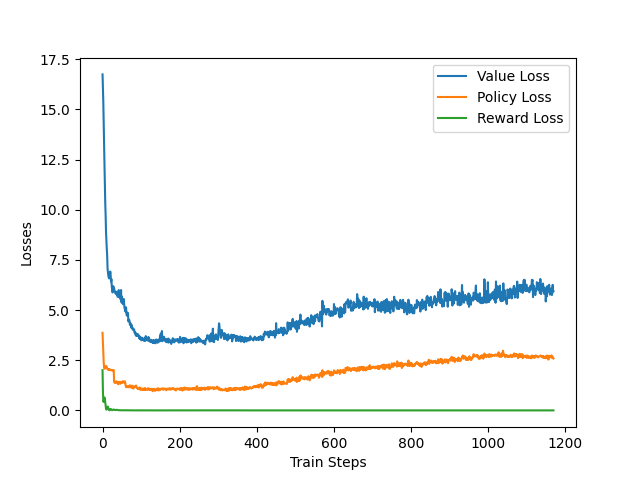
\includegraphics[width=\textwidth]{outputs/plots/sim_50/training/individual_losses.png}
    \end{minipage}
    \hfill
    \begin{minipage}{0.48\textwidth}
        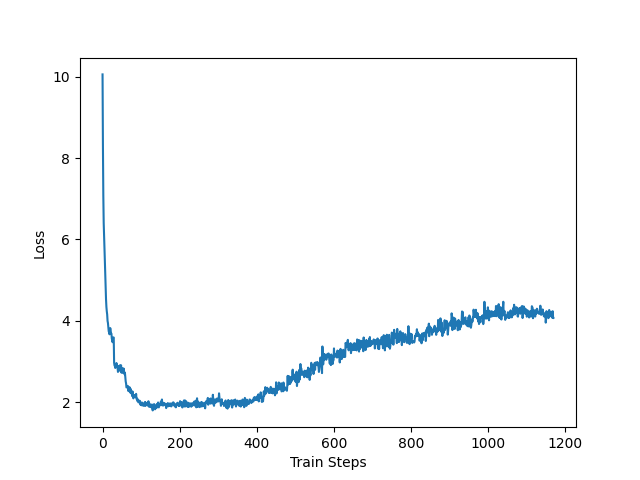
\includegraphics[width=\textwidth]{outputs/plots/sim_50/training/total_loss.png}
    \end{minipage}
    
    \vspace{1em}
    
    \begin{minipage}{0.45\textwidth}
        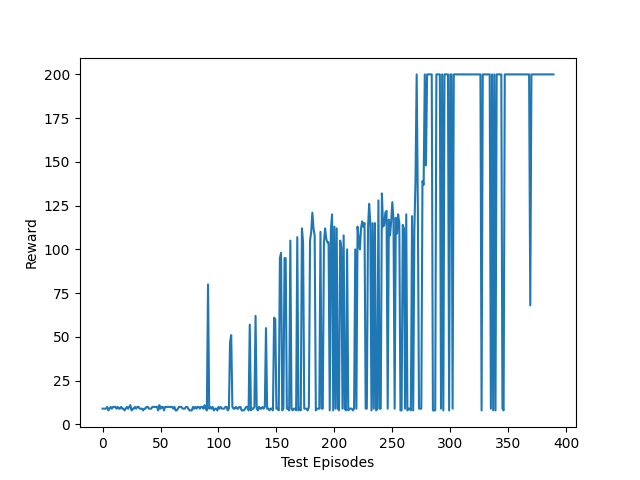
\includegraphics[width=\textwidth]{outputs/plots/sim_50/testing/test_rewards.png}
    \end{minipage}

    The policy loss initially decreases sharply in the first 100 training steps, suggesting the network quickly learns basic action preferences for the task. After the initial decline, we observe a steady increase in policy loss from around step 200 to 1200. This behavior can be attributed to more exploration as the value estimates become more reliable, the policy network adapting to complex situations as the agent learns to balance longer, and potential distribution shift as the agent encounters states it hasn't seen before. Despite rising policy loss, the test rewards plot shows consistent improving performance, reaching the maximum reward of 200 consistently by the end. This suggests that the increasing policy loss doesn't necessarily indicate worse performance, but rather reflects the complexity of the learned policy.
\end{center}
\end{tcolorbox}
\newpage

%%%%%%%%%%%%%%%%%%%%%%%%%%%%%%%%%%%%%%%%%%%%%%%%%%%%%%%%%%%%%%%%%%%%%%%%%%%

\subsection*{1.3: Effects of Hyperparameters (10 pts)}
Run MuZero with different hyperparameters and provide three plots for each value (nine total). Describe and explain the effects of the parameter.

\begin{tcolorbox}[height=45em, width=\textwidth]
    \begin{center}
        % Simulation 10 plots
        \textbf{Simulation 10} \\
        \begin{minipage}{0.32\textwidth}
            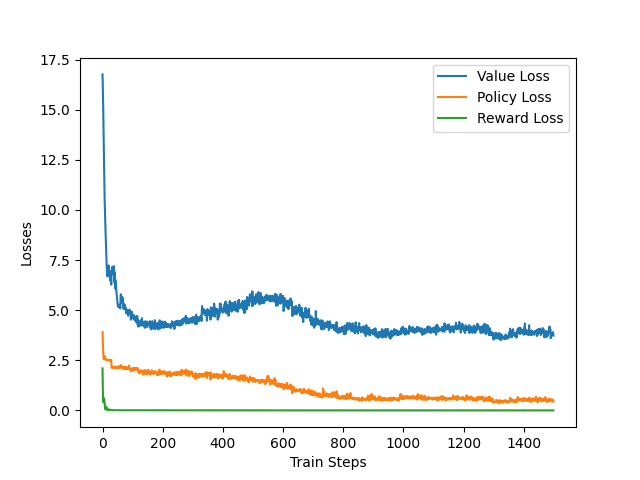
\includegraphics[width=\textwidth]{outputs/plots/sim_10/training/individual_losses.png}
        \end{minipage}%
        \hfill%
        \begin{minipage}{0.32\textwidth}
            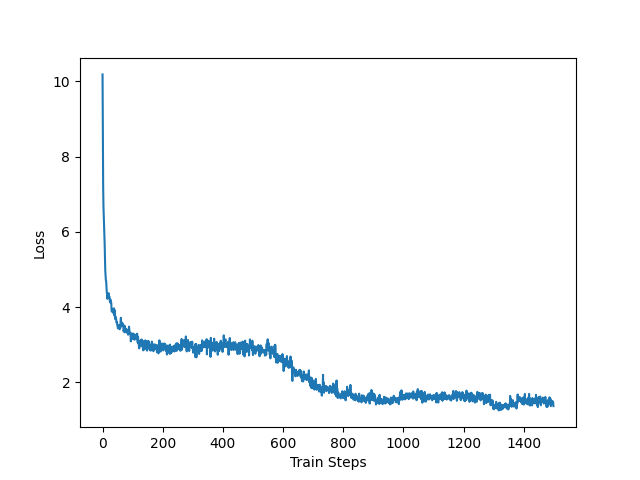
\includegraphics[width=\textwidth]{outputs/plots/sim_10/training/total_loss.png}
        \end{minipage}%
        \hfill%
        \begin{minipage}{0.32\textwidth}
            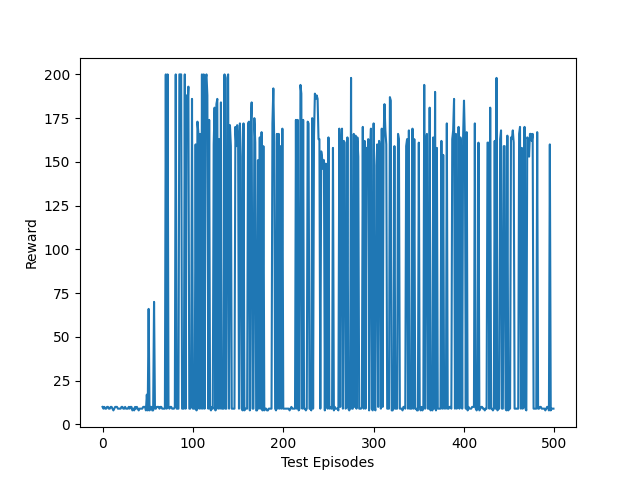
\includegraphics[width=\textwidth]{outputs/plots/sim_10/testing/test_rewards.png}
        \end{minipage}
        
        \vspace{1em}
        
        % Simulation 50 plots
        \textbf{Simulation 50} \\
        \begin{minipage}{0.32\textwidth}
            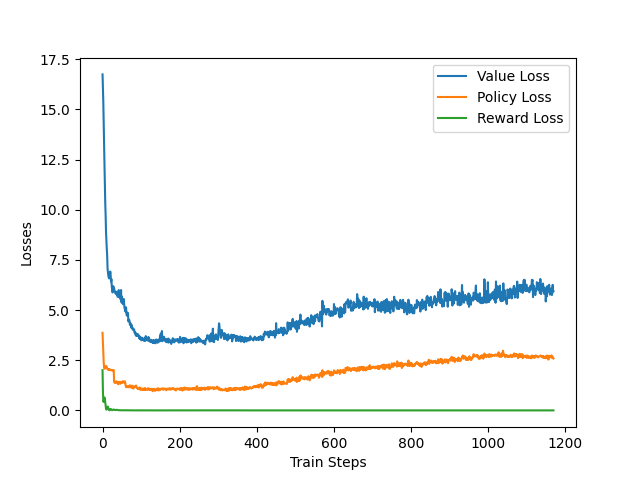
\includegraphics[width=\textwidth]{outputs/plots/sim_50/training/individual_losses.png}
        \end{minipage}%
        \hfill%
        \begin{minipage}{0.32\textwidth}
            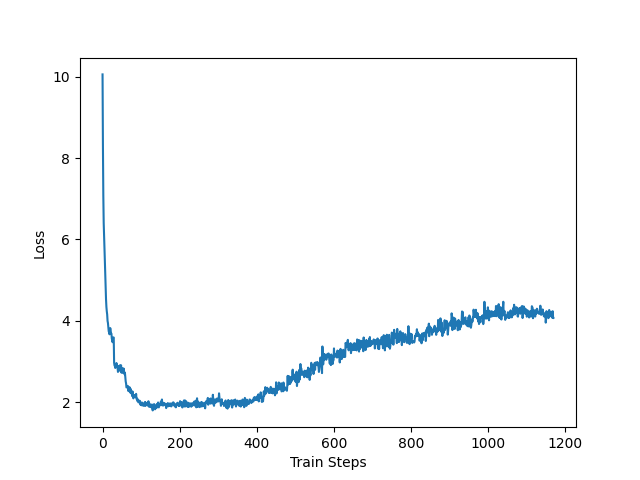
\includegraphics[width=\textwidth]{outputs/plots/sim_50/training/total_loss.png}
        \end{minipage}%
        \hfill%
        \begin{minipage}{0.32\textwidth}
            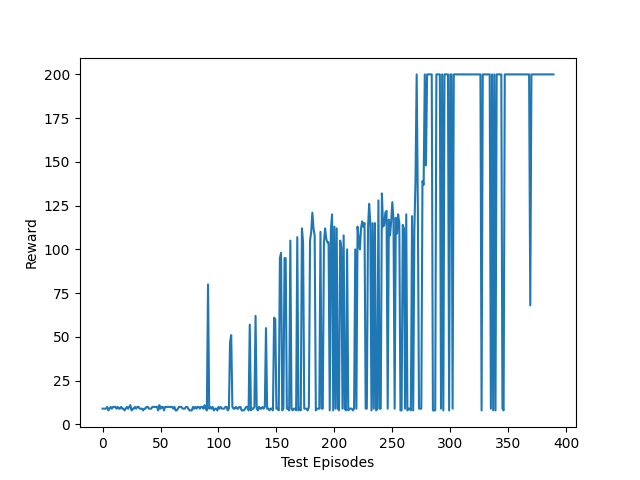
\includegraphics[width=\textwidth]{outputs/plots/sim_50/testing/test_rewards.png}
        \end{minipage}
        
        \vspace{1em}
        
        % Simulation 100 plots
        \textbf{Simulation 100} \\
        \begin{minipage}{0.32\textwidth}
            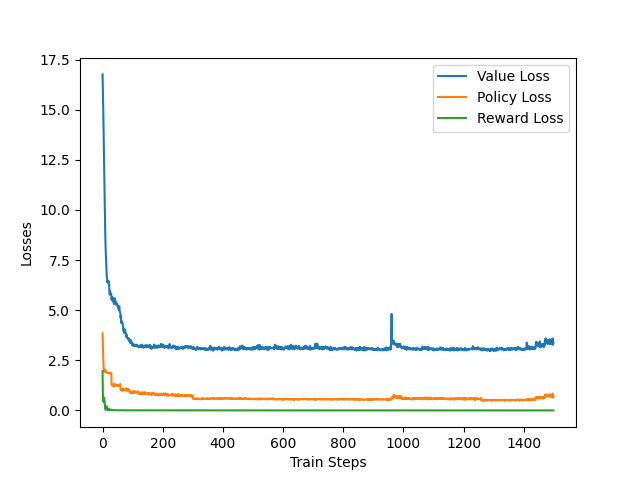
\includegraphics[width=\textwidth]{outputs/plots/sim_100/training/individual_losses.png}
        \end{minipage}%
        \hfill%
        \begin{minipage}{0.32\textwidth}
            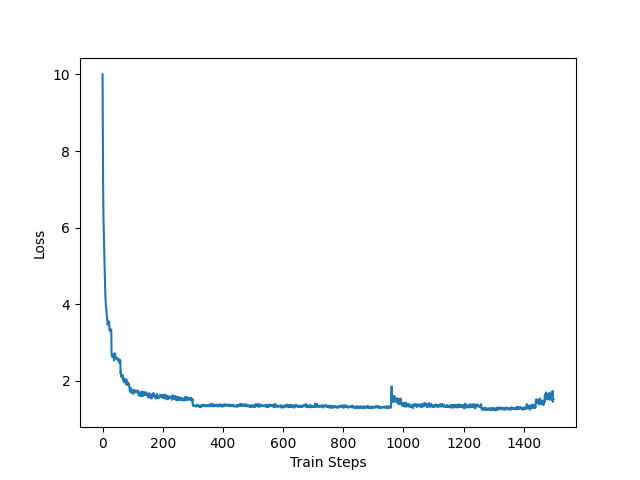
\includegraphics[width=\textwidth]{outputs/plots/sim_100/training/total_loss.png}
        \end{minipage}%
        \hfill%
        \begin{minipage}{0.32\textwidth}
            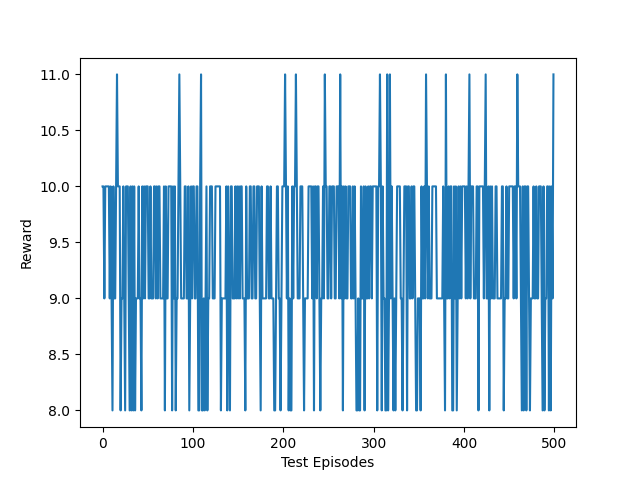
\includegraphics[width=\textwidth]{outputs/plots/sim_100/testing/test_rewards.png}
        \end{minipage}    
    \end{center}

    The number of MCTS simulations impacted training stability, with less simulations showing more volatile training and higher loss values. More simulations led to better stability with smoother loss curves. The number of simulations also impacted performance, with 50 being a good balance between exploration and exploitation, and the only one that reached the maximum reward of 200 consistently. Lower simulations had high variance in test rewards, suggesting inconsistent policy, and high simulations had lower average rewards, possibly due to over-exploration or excessive computational budget leading to conservative behavior.
\end{tcolorbox}
\newpage

%%%%%%%%%%%%%%%%%%%%%%%%%%%%%%%%%%%%%%%%%%%%%%%%%%%%%%%%%%%%%%%%%%%%%%%%%%%

\subsection*{1.4: Conceptual Questions (10 pts)}
Respond to the three questions.

\begin{tcolorbox}[height=45em, width=\textwidth]
\begin{center}
    \begin{enumerate}
        \item AlphaZero requires a known environment model, while MuZero learns the model dynamics from experience. AlphaZero works with true game states, while MuZero learns a latent state representation. AlphaZero uses the true environment for MCTS rollouts, while MuZero uses learned dynamics in latent space.
        
        MuZero would be preferred for robotics tasks where the exact physics model is unknown or complex. MuZero can learn the dynamics directly from experience, while AlphaZero would require a precise physics simulator.
    
        \item Reanalyze improves sample efficiency by revisiting old game trajectories with the latest, improved network. It uses both old and new policy targets for training, weighted by their relative quality.
        
        To implement this in the given code, we could modify \texttt{ReplayBuffer} to store full game trajectories, add a reanalyze function that runs MCTS with current network on old states, update \texttt{make\_target} to combine old and new policy targets, and add a weighting parameter to balance old vs new targets in training.
    
        \item To enforce consistency between $s_{t+1}$ and $\hat{s}_{t+1}$, we could:
        \begin{itemize}
            \item Add a consistency loss term: $L_{consist} = \|s_{t+1} - \hat{s}_{t+1}\|^2$
            \item Modify the training loop to compute both paths:
                - $s_{t+1}$ from initial inference on $o_{t+1}$
                - $\hat{s}_{t+1}$ from dynamics applied to $s_t$
            \item Add $L_{consist}$ to the total loss with appropriate weighting
            \item This would encourage the dynamics model to predict hidden states that match the representation network's output
        \end{itemize}
    \end{enumerate}    
\end{center}
\end{tcolorbox}



%%%%%%%%%%%%%%%%%%%%%%%%%%%%%%%%%%%%%%%%%%%%%%%%%%%%%%%%%%%%%%%%%%%%%%%%%%%

\clearpage
\section*{Feedback}

\textbf{Feedback}: You can help the course staff improve the course for future semesters by providing feedback. What was the most confusing part of this homework, and what would have made it less confusing?
\begin{solution}[height=4cm]
    The gym environment should be updated to a more recent version, as well as packages. Two of my teammates had M1 Macs and were unable to run the code as is. 
\end{solution}

\noindent\textbf{Time Spent}: How many hours did you spend working on this assignment? Your answer will not affect your grade. Please average your answer over all the members of your team.
\begin{table}[H]
    \centering
    \begin{tabular}{r|c}
        Alone &  \hspace{3em} 6
        \\ \hline
        With teammates & \hspace{3em} 2
        \\ \hline
        With other classmates & \hspace{3em} 0
        \\ \hline
        At office hours & \hspace{3em} 0
        \\ \hline
    \end{tabular}
\end{table}



\end{document}